\subsection{Pitch inwards and outwards force} % \label{app:...}
This test uses the test setup seen on \figref{fig:pitch_force}. The positive force is defined as a downwards direction on the load-cell.


\subsection*{Test equipment:}
\begin{itemize}
\item Endowrist model 420093 (AAU number: \#4).
\item Maxon 110160 motor with attached Maxon gearhead 110356 and Maxon encoder 201937.
\item Load cell rate for 1 kg of force \cite{Load_cell_1kg}.
\item HX711 - Load cell amplifier \cite{HX711}
\end{itemize}

\subsection*{Procedure:}
The following procedure was made:\\
Downwards force measurements:
\begin{enumerate}
\item The end-effector is rotated $90^\circ$ and attached perpendicular to the load cell. 
\item The scale is reset to zero.
\item Current is applied to the motor which control the pitch of the end-effector, at different current levels and the force is measured (downwards direction).
\item Current is increased until 1200 mA is applied.
\end{enumerate}
Step two to four is repeated five times, where the current and force is measured in respect to each other. 

Upwards force measurements:
\begin{enumerate}
\item The end-effector is rotated $90^\circ$ and attached perpendicular to the load cell. 
\item The scale is reset to zero.
\item Current is applied to the motor which control the pitch of the end-effector, at different current levels and the force is measured (upwards direction).
\item Current is increased until 1200 mA is applied.
\end{enumerate}
Step two to four is repeated five times, where the current and force is measured in respect to each other. 

\subsection*{Measuring data:}
Six of the data measurements can be seen on \figref{fig:pitch_down} and \figref{fig:pitch_up}.

\begin{figure}[H]
\centering
\input{Data/Measurement/EndoWrist_Measurements/Force/pitch_down}
\caption{Force measurements for the pitch in an downwards direction.}
\label{fig:pitch_down}
\end{figure}

\begin{figure}[H]
\centering
\input{Data/Measurement/EndoWrist_Measurements/Force/pitch_up}
\caption{Force measurements for the pitch in an upwards direction.}
\label{fig:pitch_up}
\end{figure}

%\figref{endo_force_mes}. 
%\eqref{eq:linear_force_endo}.

% \begin{equation}
% \text{y} = 0.0028 \cdot \text{x} -0.8259 
% \label{eq:linear_force_endo}
% \end{equation} 



\subsection*{Results:}
From \figref{fig:pitch_down} and \figref{fig:pitch_up} a similar pattern between the measurements can be seen. From each measurement it can be seen that the force growth for the different measurements are similar. Force is generated on the end-effector from the same current start point on both upwards and downwards measurements. It can be seen that the current is decreasing for each measurements. This is due to the controller implemented on the motor controller as it gets a setpoint and current is applied until the setpoint is reached and then decreased.
%It can be seen from the graph on \figref{endo_force_mes} that the force on the end-effector is highly nonlinear. The friction from the gearing and the Endowrist does that the force first has an exponential growth at the start. Around the 800 mA and 1200 mA step it can be seen that a drop in force is happening. What causes this drop is not identified but it can be seen that it appears for all the data sequences. \todor{better explanation?}


%% This file was created by matlab2tikz.
%
%The latest updates can be retrieved from
%  http://www.mathworks.com/matlabcentral/fileexchange/22022-matlab2tikz-matlab2tikz
%where you can also make suggestions and rate matlab2tikz.
%
\definecolor{mycolor1}{rgb}{0.00000,0.44700,0.74100}%
\definecolor{mycolor2}{rgb}{0.85000,0.32500,0.09800}%
%
\begin{figure}[h]
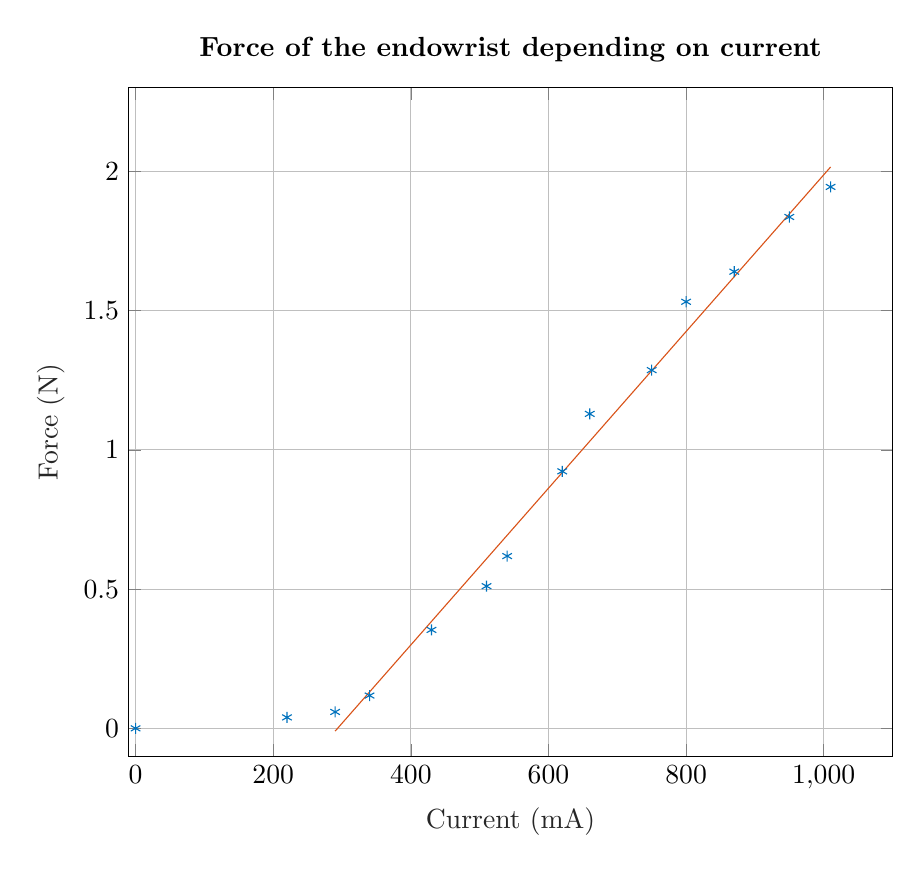
\begin{tikzpicture}

\begin{axis}[%
width=0.8\columnwidth,%7.484in,
height=0.7\columnwidth,%8.26in,
at={(0.758in,0.481in)},
scale only axis,
xmin=-10,
xmax=1100,
xlabel style={font=\color{white!15!black}},
xlabel={Current (mA)},
ymin=-0.1,
ymax=2.3,
ylabel style={font=\color{white!15!black}},
ylabel={Force (N)},
axis background/.style={fill=white},
title style={font=\bfseries},
title={Force of the endowrist depending on current},
xmajorgrids,
ymajorgrids
]
\addplot [color=mycolor1, draw=none, mark=asterisk, mark options={solid, mycolor1}, forget plot]
  table[row sep=crcr]{%
0	0\\
220	0.03928\\
290	0.05892\\
340	0.11784\\
430	0.35352\\
510	0.51064\\
540	0.61866\\
620	0.92308\\
660	1.1293\\
750	1.28642\\
800	1.53192\\
870	1.63994\\
950	1.83634\\
1010	1.94436\\
};
\addplot [color=mycolor2, forget plot]
  table[row sep=crcr]{%
290	-0.00996204344902341\\
340	0.130719594329395\\
430	0.383946542330548\\
510	0.609037162776017\\
540	0.693446145443068\\
620	0.918536765888537\\
660	1.03108207611127\\
750	1.28430902411242\\
800	1.42499066189084\\
870	1.62194495478063\\
950	1.8470355752261\\
1010	2.0158535405602\\
};
\end{axis}
\end{tikzpicture}%
\caption{The force measurements from the end-effector}
\label{endo_force_mes}
\end{figure}
\subsection*{Uncertainties of measurement:}
\begin{itemize}
\item Not 100 \% orthogonal force to the load cell.
\item Input/Output impedance of sensors have a $\pm 10 \%$ tolerance.
\item Movement of test setup when force is generated.
\end{itemize}

\subsection*{Conclusion:}
Force is generated at the end-effector when a current higher than 100 mA is applied to the motor. This is identical for all measurements. 